\documentclass[12pt]{article}
\input{/Users/joshyv/Research/misc/my_latex_defs.tex} 
%\usepackage[hypertex]{hyperref}    %for LaTeX
\usepackage{hyperref}               %for pdfLaTeX

\title{Fast Methods Comp}

\author{Joshua T. Vogelstein%\footnote{Corresponding author: joshuav@jhu.edu}
, Baktash Babidi, Liam Paninski
%$\,$ and Liam Paninski$^\#$ \\ $^\ast$ Department of Neuroscience, Johns Hopkins School of Medicine \\ $^\#$ Department of Statistics and Center for Theoretical Neuroscience, Columbia University
}

\begin{document}
\maketitle %\pagenumbering{roman}
%\setcounter{secnumdepth}{0}
%\pagenumbering{roman} %\setcounter{page}{-10}
%\pagestyle{headings}
\tableofcontents
%\listoffigures
%\listoftables

\begin{abstract}

\end{abstract}

\section{Introduction}

The goal of this work is to infer the underlying spike train, having only the observed fluorescence signal available to us.  To do so, we propose a parametric model of the experimental system.  Then, we develop a number of algorithms, each iteratively estimating the parameters and then using those parameters to infer the hidden spike trains.  

\section{Methods}
\subsection{Model}

First, for simplicity, we assume that we have extracted a time series of fluorescence observations, $F_t$, which is a function of the intracellular calcium concentration of the imaged soma at that time, $\Ca_t$.  In particular, we assume that $F_t$ simply a noisy version of $\Ca_t$, i.e.,

\begin{align} \label{eq:F}
F_t &=  \Ca_t + \varepsilon_t, \qquad \varepsilon_t \sim \mathcal{N}(0,\sigma^2),
\end{align}

\noindent where $\varepsilon_t$ is an additive Gaussian noise term with zeromean and variance $\sigma^2$. Note that this time series is naturally discrete, with time step size $\Delta$ corresponding to the frame rate of the image acquisition system, with $t$ indexing the time step, and $T$ indicating the final time step. The $\Ca$ signal is assumed to jump immediate after each spike by $A$ $\mu$M and then decay back to zero, with time constant $\tau$ sec.  Therefore, we have:

\begin{align} \label{eq:C}
\Ca_t = (1-\frac{\Delta}{\tau}) \Ca_{t-1} +  A n_t,
\end{align} 

\noindent where $n_t$ indicates the number of spikes at each time step, and is given by an exponential distribution with rate $\lambda_t$: 

\begin{align } \label{eq:n}
P(n_t|\lambda_t) = \lambda_t e^{-\lambda_t n_t \Delta}.
\end{align}

The firing rate may be any function of the stimulus, but to ensure that the likelihood of the parameters have only a single peak, we typically choose a Generalized Linear Model \ref{??,??}. Figure \ref{fig:comp} shows an example fluorescence time-series (A), the true calcium signal (B), and the true spike train (C), the expected firing rate (D) , and the stimulus (E). 
\subsection{Inferring the spike times}

We are interested in finding the spike train that caused the observed fluorescence time series.  Formally, we may be interested in computing the most likely spike train, conditioned on the fluorescence data:

\begin{align} \label{eq:lsq}
\widehat{\ve{n}} &= \argmax_{\ve{n}} P(\ve{n} | \ve{F}) =  \argmax_{\ve{n}} P(\ve{F}|\ve{n}) \p(\ve{n}) \nonumber \\ 
&=\argmax_{\ve{n}} \prod_t \p(F_t | n_t) P(n_t) = \argmax_{\ve{n}} \sum_t \log P(F_t | n_t) +
\log P(n_t) \nonumber \\
&= \argmin_{\ve{n}} \sum_t c(F_t - a
\Ca_{t-1} - A n_t)^2 + \lambda_t n_t \Delta,
\end{align}

\noindent where we let $c=1/(2\sigma^2)$ and $a=(1-\Delta/\tau)$. This is a typical regularized quadratic optimization problem, which may be solved quickly and analytically (see Appendix \ref{sec:lsq} for details). Note that this is equivalent to a Weiner filter.  However, when data is noisy, this solution tends to fit the noise as signal (see Figure 2 (B)).  As such, it is desirable to impose certain constraints on the system.  In particular, since we know that spike trains are non-negative entities, we could instead solve:

\begin{align} \label{eq:nng}
\ve{n}_{nng}&= \argmin_{\ve{n}: n_t \geq 0} \sum_t c(F_t - a \Ca_{t-1} - A n_t)^2 + \lambda_t n_t \Delta,
\end{align} 

\noindent where the only difference between \eqref{eq:lsq}and \eqref{eq:nng} is
that we've added the constraint that at each time step $n_t$ must be non-negative. Alternately, we could require that each $n_t$ is an integer:

\begin{align} \label{eq:int}
\ve{n}_{int}&= \argmin_{\ve{n}: n_t \in 0,1,2,\ldots} \sum_t c(F_t - a \Ca_{t-1} - A n_t)^2 + \lambda_t n_t \Delta.
\end{align} 

In the next subsections, we provide an efficient algorithm for solving
\eqref{eq:nng} and \eqref{eq:int}.

\subsubsection{Barrier Method}

To efficiently solve this problem, we adopt the ``barrier method''.  This approach iteratively solves a related problem that penalizes the algorithm for inferring negative values, but with each iteration, reduces the penalty, in such a way that is guaranteed to converge to \eqref{eq:nng}\ref{??}:

\begin{align} \label{eq:b}
\ve{n}_{\eta} &= \argmin_{\ve{n}} \sum_{t=0}^T c (F_t - a \Ca_{t-1} - A n_t)^2  + \lambda_t n_t - \eta \log n_t,
\end{align}

\noindent where the ``barrier term'' $-\log(n_t)$ approaches infinity as $n_t$ approaches zero. By recursively solving \eqref{eq:b}, reducing $\eta$ each time, $\ve{n}_{\eta} \rightarrow \ve{n}_{nng}$. While this function is no longer quadratic, it is still concave. Therefore, the solution may be found be iterating any gradient descent technique.  For instance, one can use Newton's method to iteratively increase the likelihood.  Importantly, the spike train may be written as a linear function of the calcium:

\begin{align}
\ve{n} &= \ma{M} \Cav \nonumber \\
\begin{bmatrix} n_0 \\ n_1 \\ \vdots \\ n_T \end{bmatrix}
= \begin{bmatrix} -a/A & 0 & 0 & \cdots \\ 1/A & -a/A & 0 & \cdots \\ \vdots \\ 0 & \cdots & 1/A & -a/A  \end{bmatrix}
\begin{bmatrix} \Ca_0 \\ \Ca_1 \\ \vdots \\ \Ca_T \end{bmatrix}
\end{align} 

\noindent where $\ma{M}$ is a bidiagonal matrix.  Therefore, \eqref{eq:b} may be solved in terms of $\Cav=\{\Ca_0, \ldots, \Ca_T\}$, by iteratively solving:

\begin{align} \label{eq:newton}
\Cav_i = \Cav_{i-1} + s \ve{d}, \qquad \ve{d}=\ma{H}^{-1}\ve{g} 
\end{align}

\noindent where $s$ is the step size, $d$ is the step direction, and $i$ indexes the iteration.  $s$ must be chosen such that all of our constraints, namely $n_t>0$ for all $t$, are satisfied:\begin{align}
0< n_t =  \ma{M}(\ve{C} + s \ve{d})
%\\ &< \ma{M} \ve{C} + s \ma{M} \ve{d}\\
\Rightarrow s > -\ma{M}\ve{C} (\ma{M} \ve{d})^{-1}. \label{eq:s}
\end{align}

Furthermore, it is possible to ''over-step'', or rather, take a step so large as to \emph{increase} the likelihood that we are trying to minimize.  As such, prior to stepping, we check that the likelihood would indeed decrease, if not, we reduce $s$ until it does. 

To compute $\ve{d}$, we must solve for the Hessian and gradient of our likelihood function with respect to $\Cav$.  Writing the likelihood in vector notation, we can solve for both: 

\begin{align}
\mathcal{L} &= c \norm{\ve{F}-\Cav}_2^2 +\ml \ma{M}\Cav - \eta \log (\ma{M}\Cav)\\
\ve{g} &=-2c(\ve{F}-\Cav)+\ve{\lambda}\ma{M} - \eta \ma{M}' (\ma{M}\Cav)^{-1} \label{eq:bar_g}\\
\ma{H} &=2c\ma{I} + 2 \eta \ma{M}' (\ma{M}\Cav)^{-2}\ma{M} \label{eq:bar_H}.
\end{align}

Plugging $\ve{g}$ and $\ma{H}$ into \eqref{eq:newton} and then choosing the step size $s$ that maximizes this likelihood, but also satisfies \eqref{eq:s} and decrease the likelihood, yields $\Cav_i$. This is iterated until it converges, at which time $\eta$ is reduced and the whole process repeats. Importantly,  the Hessian here is tridiagonal (which follows from the fact that $\ma{M}$ is bidiagonal), facilitating $O(T)$ time to solve each Newton step, as opposed to $O(T^3)$, which would be unacceptably long for large data sets.  Pseudocode for an efficient implementation of this approach is provided in Algorithm \ref{alg:bar}.  Figure \ref{fig:comp}(C) shows how this constraint further improves the inference accuracy.

\begin{algorithm}
\caption{Pseudocode for the log barrier method} \label{alg:bar}
\begin{algorithmic}
\WHILE{$\eta > \epsilon$}
\STATE Initialize $\Cav_{i}$
\STATE $\mathcal{L}_i =c \norm{\ve{F}-\Cav_i}_2^2 +\ml \ma{M}\Cav_i - \eta \log (\ma{M}\Cav_i)$
\WHILE{$\mathcal{L}_{i} < \mathcal{L}_{i-1}$}
\STATE $\ve{g}=-2c (\ve{F}-\Cav_i)+\ve{\lambda}\ma{M} - \eta \ma{M}' (\ma{M}\Cav_i)^{-1}$
\STATE $\ma{H}=2c \ma{I} + 2 \eta \ma{M}' (\ma{M}\Cav_i)^{-2}\ma{M}$
\STATE $\ve{d}=\ma{H}^{-1}\ve{g}$ efficiently
\STATE Choose $s$ such that 
\STATE $\qquad s > -\ma{M}\Cav_i (\ma{M} \ve{d})^{-1}$
\STATE $\qquad$ and $\mathcal{L}_{i} < \mathcal{L}_{i-1}$
\STATE Let $\Cav_i = \Cav_{i-1} + s \ve{d}$
\STATE $i \leftarrow i + 1$
\ENDWHILE
\STATE reduce $\eta$ 
\ENDWHILE
\end{algorithmic}
\end{algorithm}

\paragraph{Barrier Method for Intermittent data}

The barrier method may be generalized in several interesting ways.  For example, sometimes the fluorescence time-series is ``missing'' some data point due to camera mishaps, or stimulus artifacts,  for instance.  Alternately, if the precision of inferrence is higher than the frame rate, one can consider only some subset of time steps observed, and the rest missing.  In either case, one can reformulate the likelihood, gradient, and Hessian for this scenario as:

\begin{align}
\mathcal{L}&= \sum_{t=0}^T (\Ca_t - a \Ca_{t-1})^2 + f(n_t) + z_t (F_t-\Ca_t)^2 \nonumber \\
&=\norm{\Cav_t - a \Cav_{t-1}}_2^2 + f(\ve{n}) + \big(\ve{z}(\ve{F}-\Cav)\big)^2\\
\ve{g}&=2(\Cav_t - a \Cav_{t-1}) + \nabla_c f(\ve{n}) + 2 \ma{D}(\ve{z})(\ve{F}-\Cav)\\
\ma{H}&=2\ma{I} + \nabla_c^2 f(\ve{n}) + 2 \ma{D}(\ve{z})
\end{align}

\noindent where $\ve{z}=[z_0,z_T]$ takes a value $1$ during observation frames
and $0$ otherwisei, and for brevity we write the log-barrier term and the
regularizing term as $f(n_t)$, and $\ma{D}(\ve{z})$ indicates a matrix with
$\ve{z}$ along the diagonal, and zero elsewhere.

\subsubsection{Projection Pursuit Regression (PPR)}

Although the barrier method provides us with a meaningful spike train inference, we can further constrain the inferred spike train to be integers, as in \eqref{eq:int}.  Unforunately, solving this problem exactly is known to be NP-hard\ref{??}, as there are $2^T$ possible solutions.  Therefore, we instead find an approximate solution using  an algorithm called \emph{projection pursuit regression} (PPR)\ref{FS81} (see Algorithm \ref{alg:ppr} for pseudocode for this problem).  Figure \ref{fig:comp}(D) shows the inferred spike train using this algorithm. Although this approach imposes a desirable constraint (i.e., that spike trains include only integers), it also comes at a cost relative to the barrier method, as will be described in Section \ref{sec:results}.

\begin{algorithm}
\caption{Pseudocode for PPR}
\label{alg:ppr}
\begin{algorithmic}
\STATE Initialize $r^{(0)}_t=F_t, \epsilon_0 = \sum_t (r^{(0)}_t)^2$
\WHILE{$\epsilon_i<\epsilon_{i-1}$}
\STATE $t^{(i+1)}=\max_t r^{(i)} \otimes A e^{-t/\tau} + \lambda_t$
\STATE Let $\ve{o}^{(i+1)}$ be a zero vector with unity at $t^{(i+1)}$
\STATE $\Ca^{(i+1)}_t =  o^{(i+1)}_t \ast A e^{-t/\tau}$
\STATE $r^{(i+1)}_t = r^{(i)}_t -  [\ve{\text{Ca}}^{2+}]_{i+1}$
\STATE $n^{(i+1)}_t = n^{(i)}_t + o^{(i+1)}_t$
\STATE $\epsilon_{i+1} = \sum_t \big(r^{(i+1)}_t\big)^2 + \lambda_t n^{(i+1)}_t$
\ENDWHILE
\end{algorithmic}
\end{algorithm}


\subsection{Inferring the parameters}

All of the above approaches assume a particular parametric model.  As such,
these parameters must be learned.  Formally, we would like to compute:

\begin{align} \label{eq:par}
\widehat{\ve{\theta}} &= \argmax_{\ve{\theta}} \int \p(\ve{F}|\ve{n}) \p(\ve{n}) d\ve{n} \\
\{\widehat{A},\widehat{a},\widehat{c},\widehat{\ve{\lambda}}\} &= \argmax_{A,a,c,\ve{\lambda} > 0} \sum_{t=0}^T \int c(F_t - a \Ca_{t-1} - A n_t)^2 - \lambda_t n_t \Delta  dn_t
\end{align}

\noindent where $\ve{\theta}=\{A,a,c,\ve{\lambda}\}$. However, since we cannot solve the above stochastic integrals, we instead approximate \eqref{eq:par} with:

\begin{align} \label{eq:par2}
\{\widehat{A},\widehat{a},\widehat{c},\widehat{\ve{\lambda}}\} = \argmax_{A,a,c,\ve{\lambda} > 0} \sum_{t=0}^T c(F_t - a
\Ca_{t-1} - A \widehat{n}_t)^2 - \lambda_t \widehat{n}_t \Delta  
\end{align}

\noindent where $\widehat{\ve{n}}$ is the solution obtained from solving either \eqref{eq:nng} or \eqref{eq:int}.  This seems as if it should be a good approximation because the likelihood function is very high dimensional, and only a few sequences are actually likely. \eqref{eq:par2} separates out into a number of concave problems.  This may be seen by making the following subsitutions:

\begin{align*}
\Cav_{est} =\begin{bmatrix} \Cae_1\\ \vdots \\ \Cae_T \end{bmatrix},
\ve{n}_{est}=\begin{bmatrix} \widehat{n}_0\\ \vdots \\ \widehat{n}_{T-1} \end{bmatrix},
\ve{\lambda}_{est}=\begin{bmatrix} \lambda_0\\ \vdots \\ \lambda_{T-1} \end{bmatrix},
\\ \ve{F}=\begin{bmatrix} F_0\\ \vdots \\ F_{T-1} \end{bmatrix},
\ma{G}=-\begin{bmatrix} \Cav_{est}\\ \ve{n}_{est} \end{bmatrix}',
\quad \ve{x}=\begin{bmatrix} a\\ A \end{bmatrix},
\end{align*}

\noindent and plugging them into \eqref{eq:par2}:

\begin{align}
\widehat{\ve{\theta}} &=\argmin_{\ve{\theta}>\ve{0}} c\norm{\ma{G} \ve{x} + \ve{F}}_2^2 + \ve{\lambda}' \ve{n} \\
&=\argmin_{\ve{x}>\ve{0}} \frac{1}{T} (\ve{x}' \ma{G}'\ma{G} \ve{x} + 2 \ma{G}'\ve{F} \ve{x}
\end{align}

Therefore, sovling for $\widehat{\ve{x}}$ is a constrained quadratic optimization problem where $\ma{G}'\ve{G}$ is the quadratic term and $\ve{G}'\ve{F}$ is the linear term.  $c$ may be solved for analytically:

\begin{align}
\sigma^2 = \frac{1}{T} \sum_{t=0}^T (F_t - \Cae_t)^2
\end{align}

\noindent where $\Cae_t$ is the nferred $\Ca$ from either \eqref{eq:nng} or \eqref{eq:int}. Finally, $\ve{\lambda}$ may be computed by using:

\begin{align}
\lambda_t = \frac{1}{\widehat{A}\widehat{n}_t \Delta}
\end{align}

\section{Results} \label{sec:results}

Figure \ref{fig:comp}(E) shows the output of the algorithm proposed previously by Yaksi and Friedrich (2006)\ref{YF06}, which may be thought of as a custom approximation to either of these regularization approaches, and

%\section{Discussion}

\clearpage
\section{Figures}

\begin{figure}
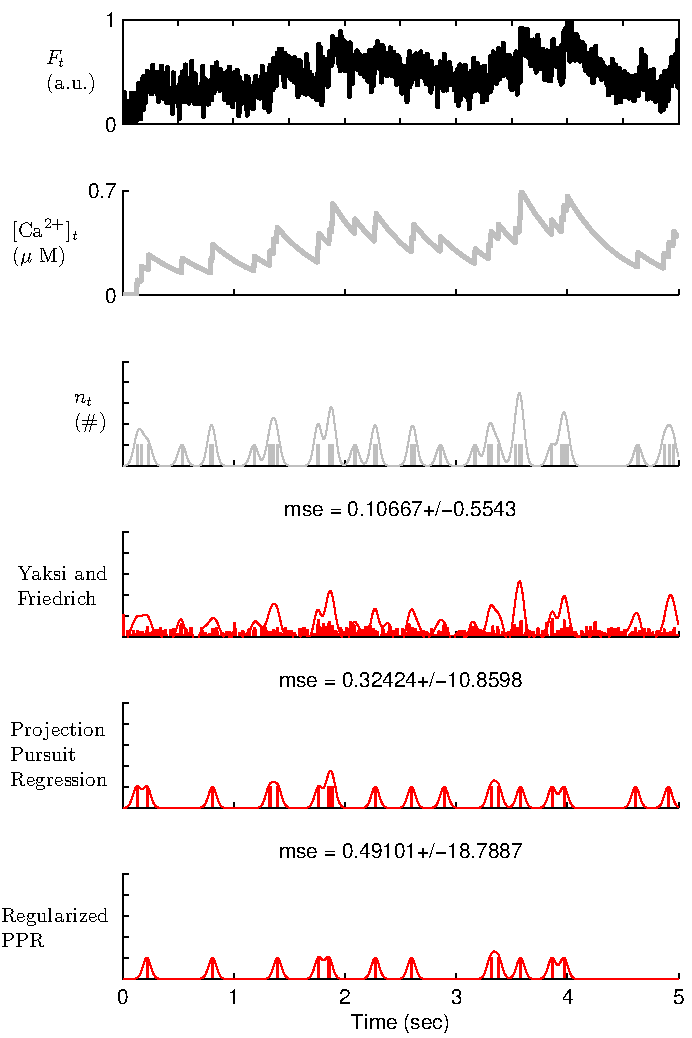
\includegraphics[width=1.0\linewidth]{comp1}
\caption{Comparison of various methods of inferring spike times. % (A) Observed fluorescence signal.  (B) True spike train.  (C) Naive inferred spike train using \eqref{eq:lsq}.  (D) Regularized spike train inference using \eqref{eq:reg}.  (E) Barrier method inferred spike train, using \eqref{eq:b}. (F) Projection pursuit regression inferred spike train, using \eqref{eq:ppr}.  All inferences used the same parameter values: $A=$ $\mu$M, $\tau=$ sec.
} \label{fig:comp}
\end{figure}


\begin{figure} \centering 
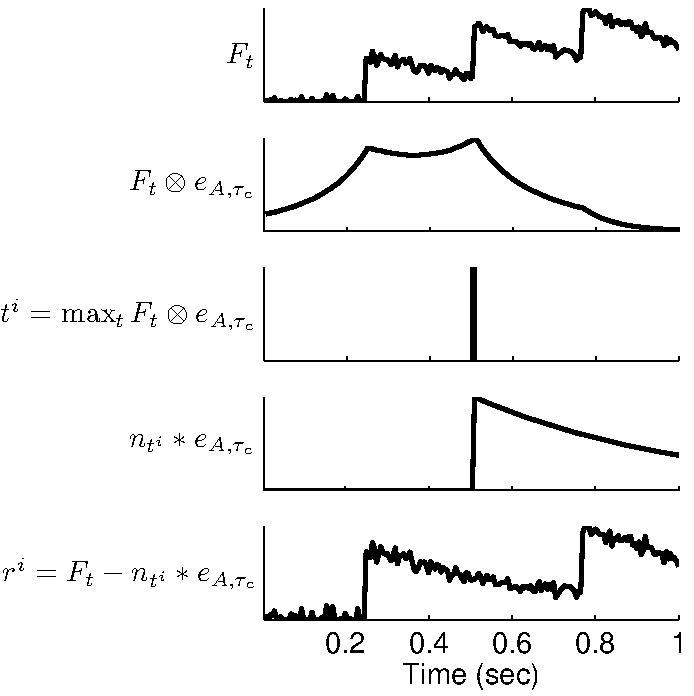
\includegraphics[height=0.8\textheight]{ppr_schem} 
\end{figure}


\newpage
\bibliography{C:/D/misc/biblist}
\addcontentsline{toc}{section}{References}
%\bibliographystyle{apalike}
\bibliographystyle{biophysj}



\end{document}
